\section{KORD Linear Regression with Multi-Airport Features: Temperature Prediction Analysis}
This analysis implements multivariate time series regression models to predict temperature at Chicago O'Hare International Airport (KORD) using weather data from multiple airports. The model incorporates both historical data and recent changes in weather patterns across all airports.\
\begin{itemize}
  \item Base Model: Multivariate Linear Regression
  \item Feature Engineering: Airport-specific features with time lags and 2-hour changes
  \item Prediction Horizons: Multiple time windows (1h, 24h, 5d, 5d avg, 30d avg)
  \item Train/Test Split: 80/20
  \item Random State: 42 (for reproducibility)
  \item Validation: Standard train-test split
\end{itemize}


\subsection{Regressors (Predictor Variables)}
Our model uses the following variables to predict KORD's temperature:

\subsubsection{KORD's Own Historical Data}
\begin{itemize}
  \item Temperature measurements from the past 24 hours (hourly lags)
  \item Temperature measurements from 48 hours ago (2-day lag)
  \item Temperature measurements from 120 hours ago (5-day lag)
  \item 5-day rolling average temperature (excluding current hour)
\end{itemize}

\subsubsection{Other Airports' Current and Historical Data}
\begin{itemize}
  \item Temperature measurements and their 24-hour lags
  \item Wind speed measurements and their 24-hour lags
  \item Wind direction measurements and their 24-hour lags
  \item Humidity measurements and their 24-hour lags
  \item Dew point measurements and their 24-hour lags
  \item Sea level pressure measurements and their 24-hour lags
  \item Visibility measurements and their 24-hour lags
  \item Cloud coverage measurements and their 24-hour lags
\end{itemize}

\subsubsection{2-Hour Change Features}
\begin{itemize}
  \item Temperature changes over the last 2 hours
  \item Wind direction changes over the last 2 hours
  \item Wind velocity changes over the last 2 hours
\end{itemize}

Each of these features is calculated for every airport in our dataset, creating a rich set of predictors that capture both local and regional weather patterns.

\subsection{Data Structure}
The dataset contains weather measurements from multiple airports, with each measurement prefixed by its airport code (e.g., KORD, KZZZ). For each airport, we track current weather measurements, 2-hour changes in key weather variables, and historical measurements through lagged features. While we use data from multiple airports, our target variable is always KORD's temperature. The other airports' data serve as potential predictors for KORD's temperature.

\subsection{Feature Engineering}
For each airport in the dataset, we create the following feature groups:

\subsubsection{Base Weather Features}
Each airport's current weather measurements include:
\begin{itemize}
  \item Temperature (°C)
  \item Wind speed (m/s)
  \item Wind direction (degrees)
  \item Humidity (\%)
  \item Dew point (°C)
  \item Sea level pressure (hPa)
  \item Visibility (km)
  \item Cloud coverage (min/max, ft)
\end{itemize}

\subsubsection{2-Hour Change Features}
For each airport, we calculate 2-hour changes in:
\begin{itemize}
  \item Temperature (\textdegree C)
  \item Wind direction (degrees)
  \item Wind velocity (m/s)
\end{itemize}

\subsubsection{Historical Features}
For each base feature, we create lagged versions at multiple time intervals:
\begin{itemize}
  \item Hourly lags (1-24 hours)
  \item 2-day lag (48 hours)
  \item 5-day lag (120 hours)
\end{itemize}
Additionally, for temperature specifically, we include a 5-day rolling average (120-hour window).

\subsection{Target Variable}
The model predicts KORD's temperature at various time horizons:
\begin{itemize}
  \item 1 hour ahead
  \item 24 hours ahead
  \item 5 days ahead
  \item 5-day average ahead
  \item 30-day average ahead
\end{itemize}

\subsection{1 Hour Ahead Temperature Prediction for KORD}
\subsection{Model Performance}
\begin{tabular}{llr}
\toprule
 & Metric & Value \\
\midrule
0 & Root Mean Squared Error (RMSE) & 0.98 \\
1 & Mean Absolute Error (MAE) & 0.58 \\
2 & R^2 Score & 0.99 \\
\bottomrule
\end{tabular}

\subsection{1 Hour Ahead Predictions}
\begin{figure}[htbp]
\centering
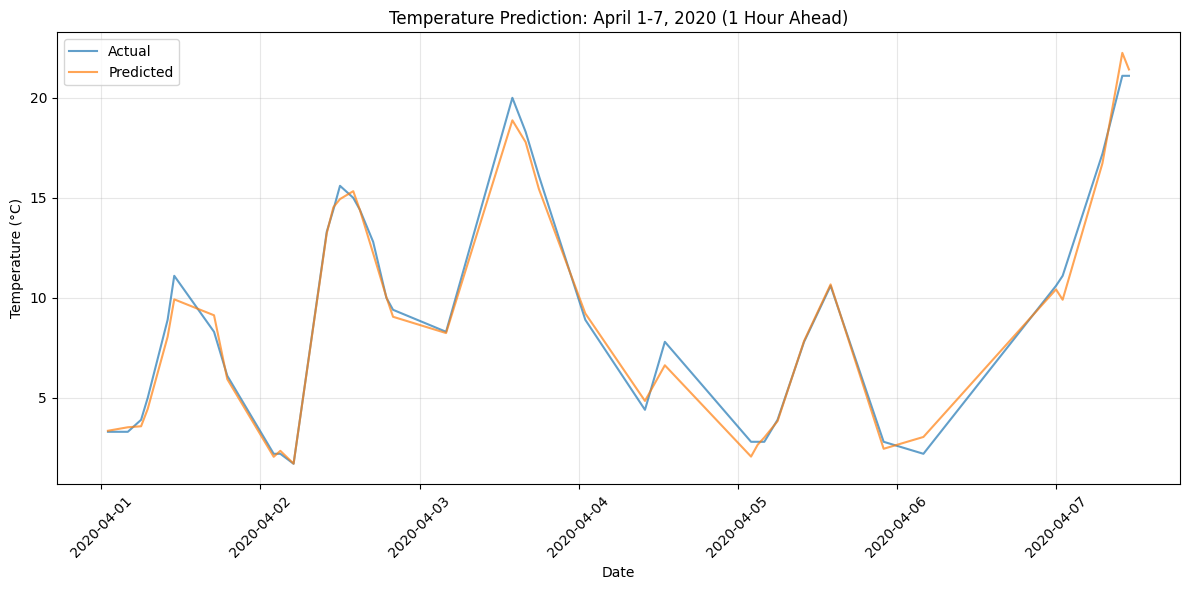
\includegraphics[width=0.7\textwidth]{1-0-linear_temp_shift_results.png}
\caption{1 Hour Ahead Predictions for KORD}
\label{fig:1_hour_ahead_pred}
\end{figure}

\subsection{1 Hour Ahead Feature Importance}
\begin{figure}[htbp]
\centering
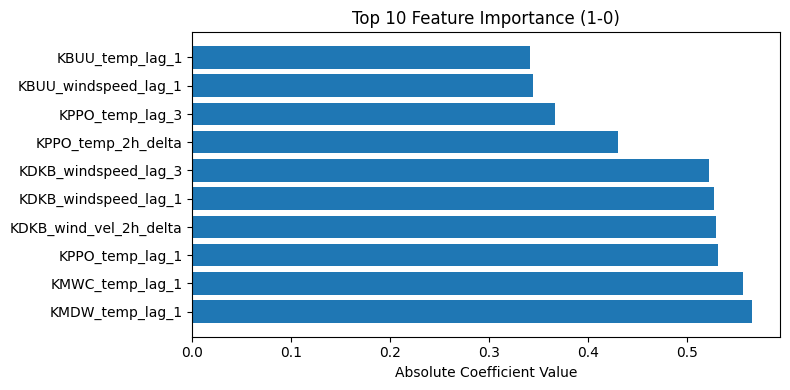
\includegraphics[width=0.7\textwidth]{1-0-linear_temp_shift_feature_importance.png}
\caption{1 Hour Ahead Feature Importance}
\label{fig:1_hour_ahead_featimp}
\end{figure}



\subsection{24 Hours Ahead Temperature Prediction for KORD}
\subsection{Model Performance}
\begin{tabular}{llr}
\toprule
 & Metric & Value \\
\midrule
0 & Root Mean Squared Error (RMSE) & 4.72 \\
1 & Mean Absolute Error (MAE) & 3.57 \\
2 & R^2 Score & 0.82 \\
\bottomrule
\end{tabular}

\subsection{24 Hours Ahead Predictions}
\begin{figure}[htbp]
\centering
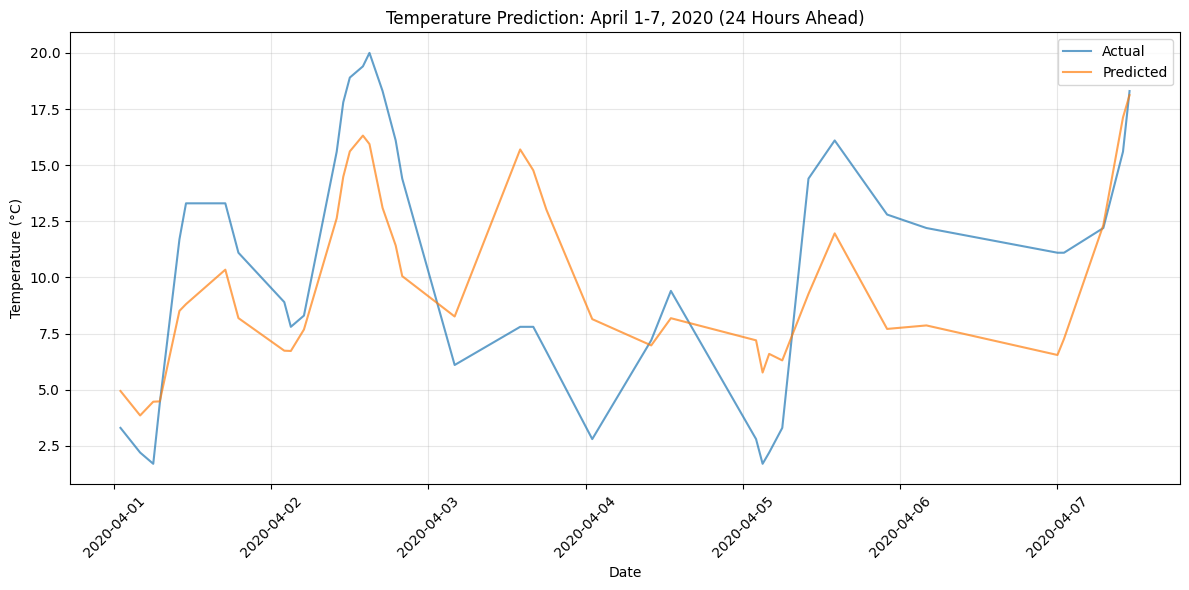
\includegraphics[width=0.7\textwidth]{1-1-linear_temp_shift_results.png}
\caption{24 Hours Ahead Predictions for KORD}
\label{fig:24_hours_ahead_pred}
\end{figure}

\subsection{24 Hours Ahead Feature Importance}
\begin{figure}[htbp]
\centering
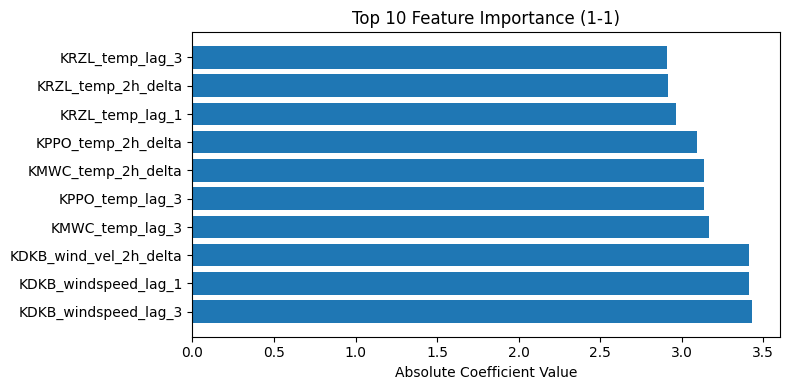
\includegraphics[width=0.7\textwidth]{1-1-linear_temp_shift_feature_importance.png}
\caption{24 Hours Ahead Feature Importance}
\label{fig:24_hours_ahead_featimp}
\end{figure}



\subsection{120 Hours (5 Days) Ahead Temperature Prediction for KORD}
\subsection{Model Performance}
\begin{tabular}{llr}
\toprule
 & Metric & Value \\
\midrule
0 & Root Mean Squared Error (RMSE) & 6.30 \\
1 & Mean Absolute Error (MAE) & 4.88 \\
2 & R^2 Score & 0.68 \\
\bottomrule
\end{tabular}

\subsection{120 Hours (5 Days) Ahead Predictions}
\begin{figure}[htbp]
\centering
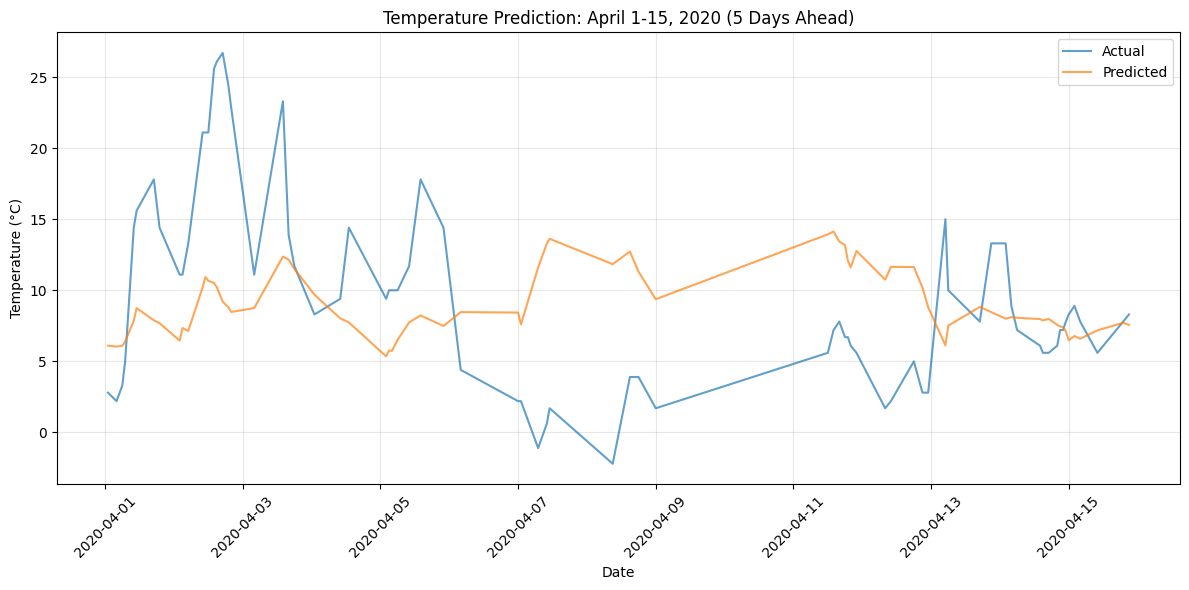
\includegraphics[width=0.7\textwidth]{1-2-linear_temp_shift_results.png}
\caption{120 Hours (5 Days) Ahead Predictions for KORD}
\label{fig:120_hours_(5_days)_ahead_pred}
\end{figure}

\subsection{120 Hours (5 Days) Ahead Feature Importance}
\begin{figure}[htbp]
\centering
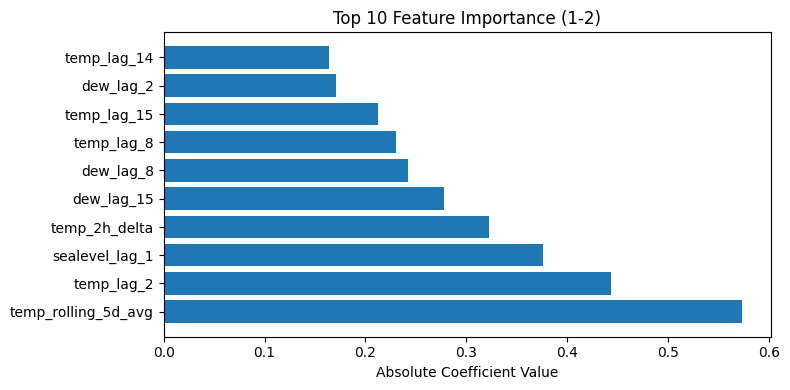
\includegraphics[width=0.7\textwidth]{1-2-linear_temp_shift_feature_importance.png}
\caption{120 Hours (5 Days) Ahead Feature Importance}
\label{fig:120_hours_(5_days)_ahead_featimp}
\end{figure}



\subsection{5-Day Average Ahead Temperature Prediction for KORD}
\subsection{Model Performance}
\begin{tabular}{llr}
\toprule
 & Metric & Value \\
\midrule
0 & Root Mean Squared Error (RMSE) & 3.64 \\
1 & Mean Absolute Error (MAE) & 2.80 \\
2 & R^2 Score & 0.87 \\
\bottomrule
\end{tabular}

\subsection{5-Day Average Ahead Predictions}
\begin{figure}[htbp]
\centering
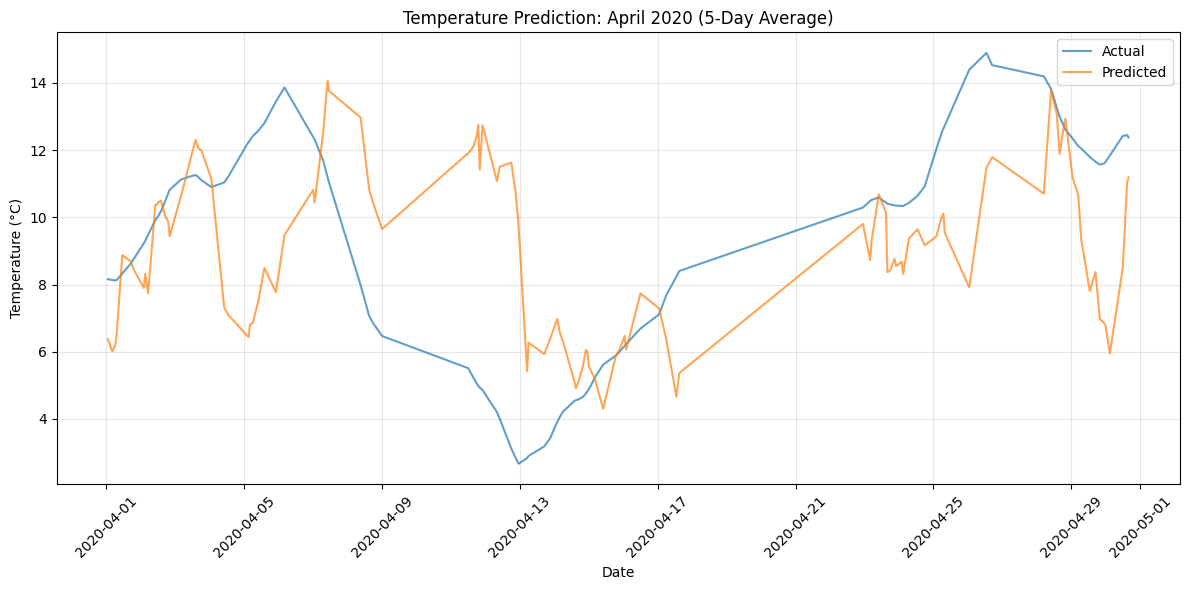
\includegraphics[width=0.7\textwidth]{1-3-linear_temp_shift_results.png}
\caption{5-Day Average Ahead Predictions for KORD}
\label{fig:5-day_average_ahead_pred}
\end{figure}

\subsection{5-Day Average Ahead Feature Importance}
\begin{figure}[htbp]
\centering
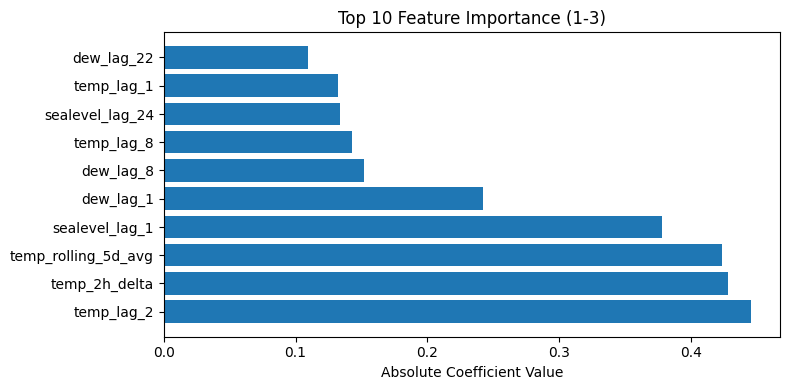
\includegraphics[width=0.7\textwidth]{1-3-linear_temp_shift_feature_importance.png}
\caption{5-Day Average Ahead Feature Importance}
\label{fig:5-day_average_ahead_featimp}
\end{figure}



\subsection{30-Day Average Ahead Temperature Prediction for KORD}
\subsection{Model Performance}
\begin{tabular}{llr}
\toprule
 & Metric & Value \\
\midrule
0 & Root Mean Squared Error (RMSE) & 4.55 \\
1 & Mean Absolute Error (MAE) & 3.67 \\
2 & R^2 Score & 0.77 \\
\bottomrule
\end{tabular}

\subsection{30-Day Average Ahead Predictions}
\begin{figure}[htbp]
\centering
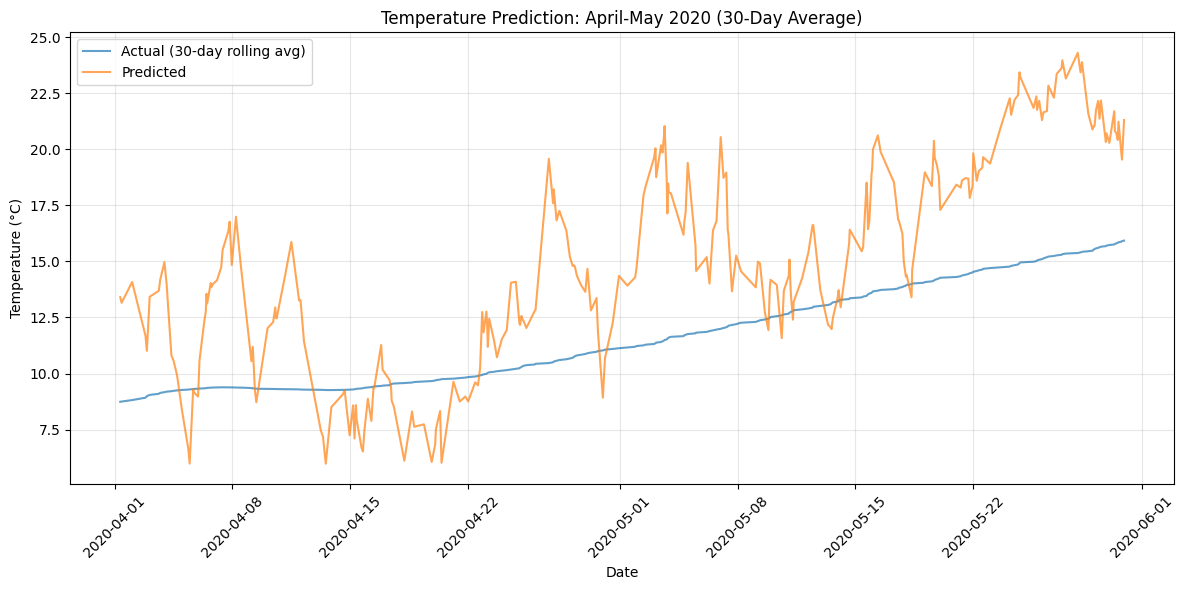
\includegraphics[width=0.7\textwidth]{1-4-linear_temp_shift_results.png}
\caption{30-Day Average Ahead Predictions for KORD}
\label{fig:30-day_average_ahead_pred}
\end{figure}

\subsection{30-Day Average Ahead Feature Importance}
\begin{figure}[htbp]
\centering
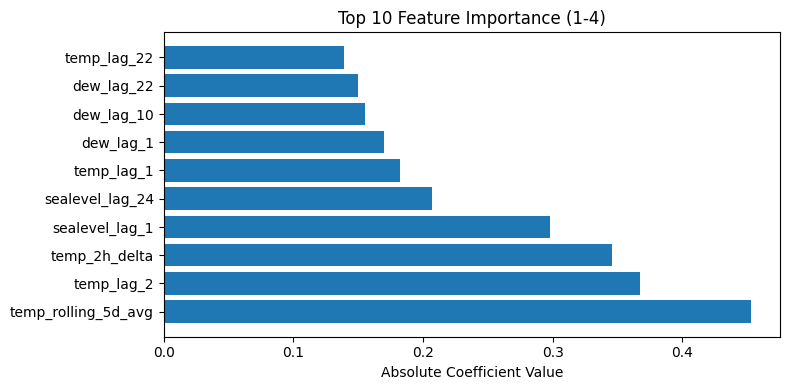
\includegraphics[width=0.7\textwidth]{1-4-linear_temp_shift_feature_importance.png}
\caption{30-Day Average Ahead Feature Importance}
\label{fig:30-day_average_ahead_featimp}
\end{figure}


\section{Model Interpretation}

These multivariate regression models capture the complex relationships between weather patterns across multiple airports and temperature at KORD. The models:\\
\begin{itemize}
  \item Use weather conditions from all available airports to predict KORD's temperature
  \item Account for recent changes in weather patterns through 2-hour delta features
  \item Incorporate historical weather patterns through lagged features
  \item Help identify which airports' weather patterns most influence KORD's temperature
\end{itemize}
Future improvements could include:\\
\begin{itemize}
  \item Feature selection to reduce dimensionality
  \item Non-linear models to capture complex relationships
  \item Time series specific models (ARIMA, LSTM)
  \item Spatial relationship modeling between airports
\end{itemize}

